% !TEX program = xelatex
% ============================================================================
% Arquitectura de microservicios por esquema (Nube + API Gateway + PostgreSQL)
% Proyecto Final de Bases de Datos - Inventario, Compras y Ventas (PostgreSQL)
% Sincronizado con Scripts sql/ y Seccion 9 del documento del proyecto.
% ============================================================================
\documentclass[tikz, border=16pt]{standalone}

\usepackage{fontspec}
\IfFontExistsTF{SourceSans3-Regular}{%
  \setmainfont{SourceSans3-Regular}[
    BoldFont = SourceSans3-Bold,
    ItalicFont = SourceSans3-It,
    BoldItalicFont = SourceSans3-BoldIt
  ]%
  \setsansfont{SourceSans3-Regular}[
    BoldFont = SourceSans3-Bold,
    ItalicFont = SourceSans3-It,
    BoldItalicFont = SourceSans3-BoldIt
  ]%
}{%
  \setmainfont{Source Sans 3}%
  \setsansfont{Source Sans 3}%
}
\IfFontExistsTF{JetBrainsMono-Regular}{%
  \setmonofont{JetBrainsMono-Regular}[
    Scale=0.86,
    BoldFont = JetBrainsMono-Bold,
    ItalicFont = JetBrainsMono-Italic
  ]%
}{%
  \setmonofont{JetBrains Mono}[Scale=0.86]%
}

\usetikzlibrary{
  arrows.meta, shapes.geometric, shapes.symbols,
  calc, shadows
}

% ---------------------------------------------------------------- paleta
\definecolor{negro}{HTML}{1F2933}
\definecolor{gris}{HTML}{3E4C59}
\definecolor{grisClaro}{HTML}{616E7C}
\definecolor{linea}{HTML}{CBD2D9}
\definecolor{fondo}{HTML}{F7F9FC}
\definecolor{acento2}{HTML}{334E68}
\definecolor{nubeFill}{HTML}{EAF4FF}
\definecolor{nubeBorder}{HTML}{3B82F6}
\definecolor{restFill}{HTML}{ECFDF5}
\definecolor{restBorder}{HTML}{10B981}

\definecolor{cCat}{HTML}{1A5DA8}   % catalogo_terceros
\definecolor{cCom}{HTML}{C96800}   % compras_abastecimiento
\definecolor{cInv}{HTML}{1E7A45}   % inventarios_transferencias
\definecolor{cVen}{HTML}{A82010}   % ventas_pagos
\definecolor{cIde}{HTML}{6030A0}   % identidad_accesos
\definecolor{cRep}{HTML}{2C3E50}   % reportes

\newcommand{\sep}{~\textperiodcentered{}\space}

% ---------------------------------------------------------------- estilos
\tikzset{
  panel/.style={
    rounded corners=10pt, draw=#1!42, fill=#1!3.5!fondo,
    line width=1.2pt
  },
  panelDash/.style={
    rounded corners=10pt, draw=#1!58, fill=#1!4!fondo,
    line width=1.3pt, dash pattern=on 7pt off 4pt
  },
  clientCard/.style={
    rounded corners=7pt, draw=acento2!55, fill=white,
    line width=1.15pt,
    drop shadow={shadow xshift=1.4pt, shadow yshift=-1.4pt,
                 fill=black!16, opacity=0.28}
  },
  svcCard/.style={
    rounded corners=7pt, draw=#1!72!black, fill=white,
    line width=1.25pt,
    drop shadow={shadow xshift=1.6pt, shadow yshift=-1.6pt,
                 fill=black!16, opacity=0.28}
  },
  dbCard/.style={
    rounded corners=7pt, draw=#1!65!black, fill=#1!5!white,
    line width=1.15pt,
    drop shadow={shadow xshift=1.4pt, shadow yshift=-1.4pt,
                 fill=black!14, opacity=0.24}
  },
  restPill/.style={
    rounded corners=3pt, draw=restBorder!85!black, fill=restFill,
    font=\sffamily\bfseries\fontsize{8.2}{9.5}\selectfont,
    text=restBorder!60!black, inner xsep=4.5pt, inner ysep=2.5pt,
    align=center
  },
  shardPill/.style={
    rounded corners=3pt, draw=#1!75!black, fill=#1!16!white,
    font=\sffamily\bfseries\fontsize{8.0}{9.2}\selectfont,
    text=#1!85!black, inner xsep=4.5pt, inner ysep=2pt
  },
  flujo/.style={-{Stealth[length=6.8pt, width=5pt]},
    draw=acento2!82, line width=1.35pt},
  flujoSvc/.style={-{Stealth[length=6.5pt, width=4.8pt]},
    draw=gris, line width=1.25pt},
  flujoD/.style={{Stealth[length=6.2pt, width=4.6pt]}%
    -{Stealth[length=6.2pt, width=4.6pt]}, draw=gris, line width=1.25pt},
  flujoDash/.style={-{Stealth[length=6.2pt, width=4.6pt]},
    draw=grisClaro, line width=1.2pt, dash pattern=on 4.5pt off 3pt},
  rotulo/.style={font=\sffamily\bfseries\fontsize{8.6}{10.2}\selectfont,
    text=negro, fill=white, inner xsep=3.5pt, inner ysep=1.5pt,
    rounded corners=2.5pt, align=center},
  port/.style={circle, draw=acento2!80, fill=white, line width=1pt,
    inner sep=0pt, minimum size=4.8pt}
}

% ---------------------------------------------------------------- iconos vectoriales
% Icono de cilindro de BD PostgreSQL centrado en (#1,#2), color #3
\newcommand{\dbicon}[3]{%
  \filldraw[fill=#3!18!white, draw=#3!82!black, line width=1.05pt]
    (#1-0.52,#2-0.46) -- (#1-0.52,#2+0.42)
    arc[start angle=180, end angle=360, x radius=0.52, y radius=0.16]
    -- (#1+0.52,#2-0.46)
    arc[start angle=360, end angle=180, x radius=0.52, y radius=0.16];
  \draw[#3!65!black, line width=0.8pt]
    (#1-0.52,#2+0.12) arc[start angle=180, end angle=360, x radius=0.52, y radius=0.15];
  \draw[#3!65!black, line width=0.8pt]
    (#1-0.52,#2-0.17) arc[start angle=180, end angle=360, x radius=0.52, y radius=0.15];
  \filldraw[fill=#3!42!white, draw=#3!82!black, line width=1.05pt]
    (#1,#2+0.42) ellipse (0.52 and 0.16);
}

% Icono hexagonal 3D de microservicio centrado en (#1,#2), color #3
\newcommand{\svcicon}[3]{%
  \node[regular polygon, regular polygon sides=6, shape border rotate=30,
        minimum size=1.08cm, fill=#3!22!white, draw=#3!85!black,
        line width=1.15pt] at (#1,#2) {};
  \draw[#3!80!black, line width=0.85pt]
    (#1,#2) -- (#1,#2-0.52)
    (#1,#2) -- (#1-0.45,#2+0.26)
    (#1,#2) -- (#1+0.45,#2+0.26);
  \fill[#3!55!white, opacity=0.45]
    (#1,#2) -- (#1-0.45,#2+0.26) -- (#1,#2+0.52) -- (#1+0.45,#2+0.26) -- cycle;
}

% Tarjeta de Microservicio (ancho 7.90 cm, alto 2.12 cm):
% \service{id}{x_left}{y_c}{color}{num}{titulo}{desc}{rol}
\newcommand{\service}[8]{%
  \node[svcCard=#4, minimum width=7.90cm, minimum height=2.12cm]
    (#1) at (#2+3.95,#3) {};
  \fill[#4!82!black, rounded corners=2pt]
    (#2+0.14,#3+0.88) rectangle (#2+7.76,#3+0.96);
  \svcicon{#2+0.78}{#3-0.02}{#4}
  \node[anchor=west, text=#4!85!black,
        font=\sffamily\bfseries\fontsize{9.5}{11}\selectfont]
    at (#2+1.44,#3+0.58) {#5\enspace\textperiodcentered{}\enspace\fontsize{12.2}{14.2}\selectfont #6};
  \node[anchor=north west, text=negro,
        font=\sffamily\fontsize{9.6}{11.8}\selectfont,
        text width=6.25cm, align=left]
    at (#2+1.44,#3+0.34) {\raggedright #7};
  \node[anchor=west, text=gris,
        font=\sffamily\fontsize{9.2}{11}\selectfont]
    at (#2+1.44,#3-0.72) {Propietario:\enspace{\ttfamily\bfseries\color{#4!85!black}#8}};
}

% Cilindro / Esquema PostgreSQL (ancho 9.00 cm, alto 2.12 cm):
% \dbschema{id}{x_left}{y_c}{color}{esquema}{tablas}{nota}{badge}
\newcommand{\dbschema}[8]{%
  \node[dbCard=#4, minimum width=9.00cm, minimum height=2.12cm]
    (#1) at (#2+4.50,#3) {};
  \dbicon{#2+0.80}{#3}{#4}
  \node[anchor=west, font=\ttfamily\bfseries\fontsize{10.8}{13}\selectfont,
        text=#4!85!black]
    at (#2+1.52,#3+0.60) {#5};
  \node[anchor=west, text=negro,
        font=\sffamily\fontsize{9.4}{11.4}\selectfont,
        text width=7.20cm, align=left]
    at (#2+1.52,#3-0.02) {\raggedright #6};
  \node[anchor=west, text=gris,
        font=\sffamily\fontsize{8.9}{10.8}\selectfont]
    at (#2+1.52,#3-0.68) {#7};
  \if\relax\detokenize{#8}\relax\else
    \node[shardPill=#4, anchor=south east]
      at (#2+8.84,#3-0.88) {#8};
  \fi
}

% ============================================================================
\begin{document}
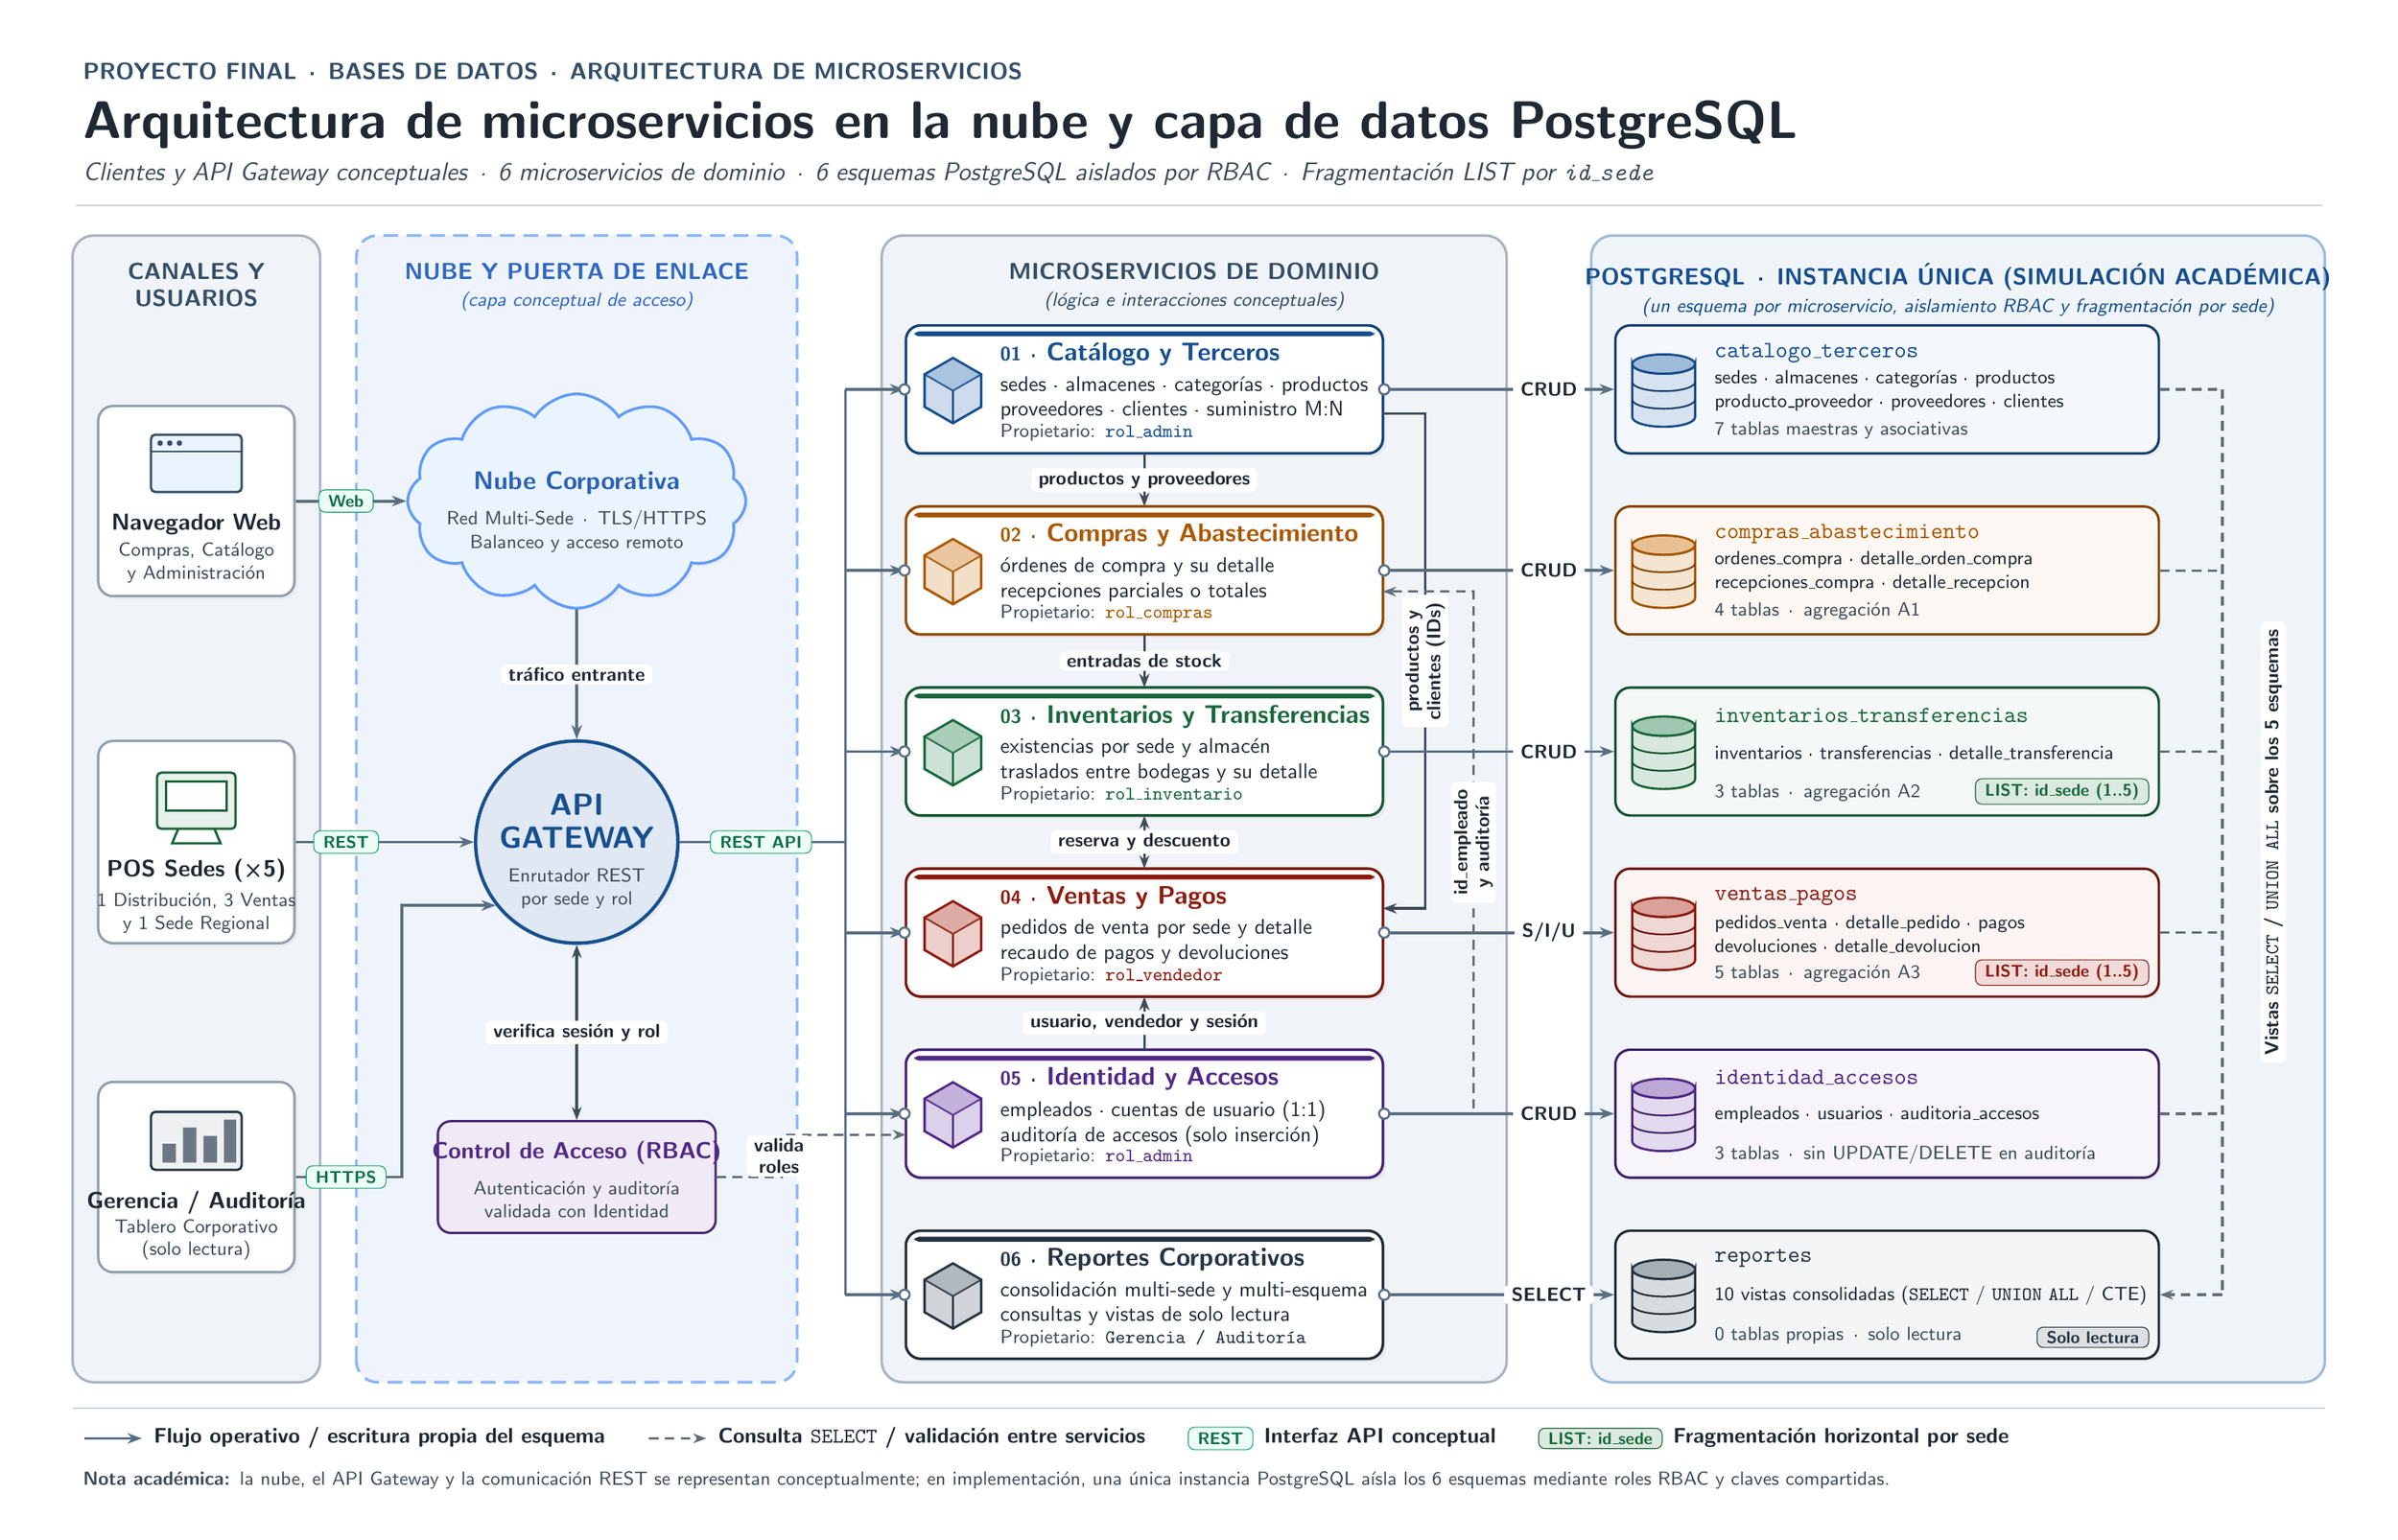
\begin{tikzpicture}
\path[use as bounding box] (0,0) rectangle (39.0,24.8);

% ====================================================================
% ENCABEZADO
% ====================================================================
\node[anchor=west, text=acento2,
      font=\sffamily\bfseries\fontsize{10.5}{12.5}\selectfont]
  at (0.9,23.95)
  {PROYECTO FINAL\enspace\textperiodcentered\enspace BASES DE DATOS\enspace\textperiodcentered\enspace ARQUITECTURA DE MICROSERVICIOS};

\node[anchor=west, text=negro,
      font=\sffamily\bfseries\fontsize{25}{29}\selectfont]
  at (0.9,23.08)
  {Arquitectura de microservicios en la nube y capa de datos PostgreSQL};

\node[anchor=west, text=gris,
      font=\sffamily\itshape\fontsize{12.2}{15}\selectfont]
  at (0.9,22.26)
  {Clientes y API Gateway conceptuales\enspace\textperiodcentered\enspace
   6 microservicios de dominio\enspace\textperiodcentered\enspace
   6 esquemas PostgreSQL aislados por RBAC\enspace\textperiodcentered\enspace
   Fragmentaci\'on LIST por \texttt{id\_sede}};

\draw[linea, line width=0.8pt] (0.9,21.75) -- (38.1,21.75);

% ====================================================================
% FONDOS DE CAPAS ARQUITECTONICAS
% ====================================================================
% Capa 1: Canales / Clientes
\draw[panel=acento2] (0.85,2.25) rectangle (4.95,21.25);
\node[anchor=north, text=acento2,
      font=\sffamily\bfseries\fontsize{11}{13}\selectfont, align=center]
  at (2.90,20.92) {CANALES Y\\USUARIOS};

% Capa 2: Nube y API Gateway (conceptual)
\draw[panelDash=nubeBorder] (5.55,2.25) rectangle (12.85,21.25);
\node[anchor=north, text=nubeBorder!80!black,
      font=\sffamily\bfseries\fontsize{11}{13}\selectfont, align=center]
  at (9.20,20.92) {NUBE Y PUERTA DE ENLACE\\{\fontsize{9}{11}\selectfont\mdseries\itshape(capa conceptual de acceso)}};

% Capa 3: Microservicios de dominio
\draw[panel=acento2] (14.25,2.25) rectangle (24.60,21.25);
\node[anchor=north, text=acento2,
      font=\sffamily\bfseries\fontsize{11}{13}\selectfont, align=center]
  at (19.425,20.92) {MICROSERVICIOS DE DOMINIO\\{\fontsize{9}{11}\selectfont\mdseries\itshape(l\'ogica e interacciones conceptuales)}};

% Capa 4: PostgreSQL instancia unica
\draw[panel=cCat] (26.00,2.25) rectangle (38.15,21.25);
\node[anchor=north, text=cCat!85!black,
      font=\sffamily\bfseries\fontsize{11}{13}\selectfont, align=center]
  at (32.075,20.92) {POSTGRESQL\enspace·\enspace INSTANCIA \'UNICA (SIMULACI\'ON ACAD\'EMICA)\\{\fontsize{9}{11}\selectfont\mdseries\itshape(un esquema por microservicio, aislamiento RBAC y fragmentaci\'on por sede)}};

% ====================================================================
% CAPA 1: CLIENTES (Columna izquierda)
% ====================================================================
% Cliente 1: Navegador Web (alineado con Nube y = 16.85)
\node[clientCard, minimum width=3.25cm, minimum height=3.15cm] (cliWeb) at (2.90,16.85) {};
\draw[acento2, line width=1.1pt, rounded corners=2pt, fill=nubeFill]
  (2.15,17.00) rectangle (3.65,17.95);
\draw[acento2, line width=0.9pt] (2.15,17.67) -- (3.65,17.67);
\fill[acento2] (2.30,17.81) circle (1.3pt) (2.46,17.81) circle (1.3pt) (2.62,17.81) circle (1.3pt);
\node[text=negro, font=\sffamily\bfseries\fontsize{10.5}{12.5}\selectfont]
  at (2.90,16.47) {Navegador Web};
\node[text=gris, font=\sffamily\fontsize{8.8}{10.8}\selectfont, align=center]
  at (2.90,15.83) {Compras, Cat\'alogo\\y Administraci\'on};

% Cliente 2: POS Sedes (x5) (alineado con API Gateway y = 11.20)
\node[clientCard, minimum width=3.25cm, minimum height=3.35cm] (cliPos) at (2.90,11.20) {};
\draw[cInv!80!black, line width=1.1pt, rounded corners=2pt, fill=cInv!10]
  (2.25,11.42) rectangle (3.55,12.35);
\draw[cInv!80!black, line width=1.0pt, fill=white]
  (2.40,11.72) rectangle (3.40,12.20);
\draw[cInv!80!black, line width=1.1pt] (2.60,11.42) -- (2.50,11.18) -- (3.30,11.18) -- (3.20,11.42);
\node[text=negro, font=\sffamily\bfseries\fontsize{10.5}{12.5}\selectfont]
  at (2.90,10.72) {POS Sedes (\texttimes 5)};
\node[text=gris, font=\sffamily\fontsize{8.8}{10.8}\selectfont, align=center]
  at (2.90,10.02) {1 Distribuci\'on, 3 Ventas\\y 1 Sede Regional};

% Cliente 3: Portal Gerencia y Auditoria (alineado con RBAC y = 5.65)
\node[clientCard, minimum width=3.25cm, minimum height=3.15cm] (cliGer) at (2.90,5.65) {};
\draw[cRep!85!black, line width=1.1pt, rounded corners=2pt, fill=cRep!8]
  (2.15,5.77) rectangle (3.65,6.73);
\fill[cRep!70] (2.34,5.89) rectangle (2.56,6.20)
               (2.68,5.89) rectangle (2.90,6.47)
               (3.02,5.89) rectangle (3.24,6.33)
               (3.36,5.89) rectangle (3.56,6.60);
\node[text=negro, font=\sffamily\bfseries\fontsize{10.5}{12.5}\selectfont]
  at (2.90,5.23) {Gerencia / Auditor\'ia};
\node[text=gris, font=\sffamily\fontsize{8.8}{10.8}\selectfont, align=center]
  at (2.90,4.61) {Tablero Corporativo\\(solo lectura)};

% ====================================================================
% CAPA 2: NUBE + API GATEWAY (conceptual)
% ====================================================================
% Nube superior
\node[cloud, cloud puffs=12, cloud puff arc=115, aspect=1.75,
      draw=nubeBorder!80, fill=nubeFill, line width=1.3pt,
      minimum width=5.6cm, minimum height=3.55cm,
      drop shadow={shadow xshift=1.5pt, shadow yshift=-1.5pt,
                   fill=black!14, opacity=0.22}]
  (nube) at (9.20,16.85) {};
\node[text=nubeBorder!75!black,
      font=\sffamily\bfseries\fontsize{12.5}{14.5}\selectfont, align=center]
  at (9.20,17.15) {Nube Corporativa};
\node[text=gris, font=\sffamily\fontsize{9.2}{11.2}\selectfont, align=center]
  at (9.20,16.35) {Red Multi-Sede\enspace·\enspace TLS/HTTPS\\Balanceo y acceso remoto};

% Hub API Gateway
\node[circle, draw=cCat!85!black, fill=cCat!14!white, line width=1.6pt,
      minimum size=3.35cm,
      drop shadow={shadow xshift=1.6pt, shadow yshift=-1.6pt,
                   fill=black!16, opacity=0.26}]
  (gw) at (9.20,11.20) {};
\node[text=cCat!85!black,
      font=\sffamily\bfseries\fontsize{13.5}{15.5}\selectfont, align=center]
  at (9.20,11.55) {API\\GATEWAY};
\node[text=gris, font=\sffamily\fontsize{8.8}{10.8}\selectfont, align=center]
  at (9.20,10.43) {Enrutador REST\\por sede y rol};

% Modulo transversal RBAC dentro de la nube
\node[rounded corners=6pt, draw=cIde!75!black, fill=cIde!10!white,
      line width=1.1pt, minimum width=4.6cm, minimum height=1.85cm]
  (authBox) at (9.20,5.65) {};
\node[text=cIde!85!black,
      font=\sffamily\bfseries\fontsize{10.5}{12.5}\selectfont, align=center]
  at (9.20,6.05) {Control de Acceso (RBAC)};
\node[text=gris, font=\sffamily\fontsize{8.8}{10.8}\selectfont, align=center]
  at (9.20,5.28) {Autenticaci\'on y auditor\'ia\\validada con Identidad};

% Conexiones Clientes -> Nube -> API Gateway
\draw[flujo] (cliWeb.east) -- (nube.west);
\node[restPill] at (5.38,16.85) {Web};

\draw[flujo] (cliPos.east) -- (gw.west);
\node[restPill] at (5.38,11.20) {REST};

\draw[flujo] (cliGer.east) -- (6.30,5.65) -- (6.30,10.15) -- (7.86,10.15);
\node[restPill] at (5.38,5.65) {HTTPS};

\draw[flujo] (nube.south) -- node[rotulo, pos=0.5]{tr\'afico entrante} (gw.north);
\draw[flujoD] (gw.south) -- node[rotulo, pos=0.5]{verifica sesi\'on y rol} (authBox.north);

% ====================================================================
% CAPA 3: 6 MICROSERVICIOS DE DOMINIO (orden logico 01..06)
% y = 18.7, 15.7, 12.7, 9.7, 6.7, 3.7
% ====================================================================
\service{svcCat}{14.65}{18.70}{cCat}{01}{Cat\'alogo y Terceros}
  {sedes\sep almacenes\sep categor\'ias\sep productos\\proveedores\sep clientes\sep suministro M:N}
  {rol\_admin}

\service{svcCom}{14.65}{15.70}{cCom}{02}{Compras y Abastecimiento}
  {\'ordenes de compra y su detalle\\recepciones parciales o totales}
  {rol\_compras}

\service{svcInv}{14.65}{12.70}{cInv}{03}{Inventarios y Transferencias}
  {existencias por sede y almac\'en\\traslados entre bodegas y su detalle}
  {rol\_inventario}

\service{svcVen}{14.65}{9.70}{cVen}{04}{Ventas y Pagos}
  {pedidos de venta por sede y detalle\\recaudo de pagos y devoluciones}
  {rol\_vendedor}

\service{svcIde}{14.65}{6.70}{cIde}{05}{Identidad y Accesos}
  {empleados\sep cuentas de usuario (1:1)\\auditor\'ia de accesos (solo inserci\'on)}
  {rol\_admin}

\service{svcRep}{14.65}{3.70}{cRep}{06}{Reportes Corporativos}
  {consolidaci\'on multi-sede y multi-esquema\\consultas y vistas de solo lectura}
  {Gerencia / Auditor\'ia}

% Bus REST API desde API Gateway hacia los 6 microservicios
\draw[acento2!80, line width=1.4pt] (gw.east) -- (13.65,11.20);
\node[restPill] at (12.25,11.20) {REST API};
\draw[acento2!80, line width=1.4pt] (13.65,3.70) -- (13.65,18.70);

\foreach \svc/\yc in {
  svcCat/18.70, svcCom/15.70, svcInv/12.70,
  svcVen/9.70,  svcIde/6.70,  svcRep/3.70} {
  \draw[flujo] (13.65,\yc) -- (\svc.west);
  \node[port] at (\svc.west) {};
}

% Validacion RBAC directa hacia 05 Identidad (sin cruzar la linea REST API!)
\draw[flujoDash] (authBox.east) -- (12.60,5.65) -- (12.60,6.35) -- (14.65,6.35);
\node[rotulo] at (12.55,6.00) {valida\\roles};

% ====================================================================
% INTERACCIONES CONCEPTUALES ENTRE MICROSERVICIOS
% ====================================================================
% 01 Catalogo -> 02 Compras
\draw[flujoSvc] (18.60,17.64) -- (18.60,16.76);
\node[rotulo] at (18.60,17.20) {productos y proveedores};

% 02 Compras -> 03 Inventarios
\draw[flujoSvc] (18.60,14.64) -- (18.60,13.76);
\node[rotulo] at (18.60,14.20) {entradas de stock};

% 03 Inventarios <-> 04 Ventas
\draw[flujoD] (18.60,11.64) -- (18.60,10.76);
\node[rotulo] at (18.60,11.20) {reserva y descuento};

% 05 Identidad -> 04 Ventas
\draw[flujoSvc] (18.60,7.76) -- (18.60,8.64);
\node[rotulo] at (18.60,8.20) {usuario, vendedor y sesi\'on};

% 01 Catalogo -> 04 Ventas (corredor derecho de Capa 3, x = 23.25)
\draw[flujoSvc] (22.55,18.30) -- (23.25,18.30) -- (23.25,10.10) -- (22.55,10.10);
\node[rotulo, rotate=90] at (23.25,14.20) {productos y\\clientes (IDs)};

% 05 Identidad -> 02 Compras (corredor derecho de Capa 3, x = 24.05)
\draw[flujoDash] (22.55,6.70) -- (24.05,6.70) -- (24.05,15.35) -- (22.55,15.35);
\node[rotulo, rotate=90] at (24.05,11.20) {id\_empleado\\y auditor\'ia};

% ====================================================================
% CAPA 4: POSTGRESQL INSTANCIA UNICA (6 cilindros de esquema)
% ====================================================================
\dbschema{dbCat}{26.40}{18.70}{cCat}{catalogo\_terceros}
  {sedes\sep almacenes\sep categor\'ias\sep productos\\producto\_proveedor\sep proveedores\sep clientes}
  {7 tablas maestras y asociativas}{}

\dbschema{dbCom}{26.40}{15.70}{cCom}{compras\_abastecimiento}
  {ordenes\_compra\sep detalle\_orden\_compra\\recepciones\_compra\sep detalle\_recepcion}
  {4 tablas\enspace·\enspace agregaci\'on A1}{}

\dbschema{dbInv}{26.40}{12.70}{cInv}{inventarios\_transferencias}
  {inventarios\sep transferencias\sep detalle\_transferencia}
  {3 tablas\enspace·\enspace agregaci\'on A2}{LIST: id\_sede (1..5)}

\dbschema{dbVen}{26.40}{9.70}{cVen}{ventas\_pagos}
  {pedidos\_venta\sep detalle\_pedido\sep pagos\\devoluciones\sep detalle\_devolucion}
  {5 tablas\enspace·\enspace agregaci\'on A3}{LIST: id\_sede (1..5)}

\dbschema{dbIde}{26.40}{6.70}{cIde}{identidad\_accesos}
  {empleados\sep usuarios\sep auditoria\_accesos}
  {3 tablas\enspace·\enspace sin UPDATE/DELETE en auditor\'ia}{}

\dbschema{dbRep}{26.40}{3.70}{cRep}{reportes}
  {10 vistas consolidadas (\texttt{SELECT} / \texttt{UNION ALL} / CTE)}
  {0 tablas propias\enspace·\enspace solo lectura}{Solo lectura}

% Conexiones Microservicio -> Su propio Esquema PostgreSQL (propiedad estricta)
\foreach \svc/\db/\yc/\lbl in {
  svcCat/dbCat/18.70/CRUD,
  svcCom/dbCom/15.70/CRUD,
  svcInv/dbInv/12.70/CRUD,
  svcVen/dbVen/9.70/{S/I/U},
  svcIde/dbIde/6.70/CRUD,
  svcRep/dbRep/3.70/SELECT} {
  \draw[flujo] (\svc.east) -- (\db.west);
  \node[port] at (\svc.east) {};
  \node[rotulo] at (25.30,\yc) {\lbl};
}

% Bus de consolidacion de solo lectura hacia esquema reportes (x = 36.45)
\draw[grisClaro, line width=1.25pt, dash pattern=on 4.5pt off 3pt]
  (36.45,18.70) -- (36.45,3.70);
\foreach \db/\yc in {
  dbCat/18.70, dbCom/15.70, dbInv/12.70, dbVen/9.70, dbIde/6.70} {
  \draw[grisClaro, line width=1.2pt, dash pattern=on 4.5pt off 3pt]
    (\db.east) -- (36.45,\yc);
}
\draw[flujoDash] (36.45,3.70) -- (dbRep.east);
\node[rotulo, rotate=90] at (37.30,11.20)
  {Vistas \texttt{SELECT} / \texttt{UNION ALL} sobre los 5 esquemas};

% ====================================================================
% PIE / LEYENDA
% ====================================================================
\draw[linea, line width=0.8pt] (0.85,1.82) -- (38.15,1.82);

\node[anchor=west, text=negro, font=\sffamily\fontsize{9.6}{12}\selectfont]
  at (0.90,1.32) {%
  \tikz[baseline=-0.5ex]{\draw[flujo] (0,0)--(0.95,0);}\enspace
  \textbf{Flujo operativo / escritura propia del esquema}\qquad
  \tikz[baseline=-0.5ex]{\draw[flujoDash] (0,0)--(0.95,0);}\enspace
  \textbf{Consulta \texttt{SELECT} / validaci\'on entre servicios}\qquad
  \tikz[baseline=-0.5ex]{\node[restPill]{REST};}\enspace
  \textbf{Interfaz API conceptual}\qquad
  \tikz[baseline=-0.5ex]{\node[shardPill=cInv]{LIST: id\_sede};}\enspace
  \textbf{Fragmentaci\'on horizontal por sede}};

\node[anchor=west, text=gris, font=\sffamily\fontsize{9.4}{11.5}\selectfont]
  at (0.90,0.62) {%
  \textbf{Nota acad\'emica:}\enspace la nube, el API Gateway y la comunicaci\'on REST se representan conceptualmente; en implementaci\'on, una \'unica instancia PostgreSQL a\'isla los 6 esquemas mediante roles RBAC y claves compartidas.};

\end{tikzpicture}
\end{document}
